\chapter{Event Detection Using Event-Driven Multiple Instance Learning}
\label{chapter5}
%\setlength{\epigraphrule}{0pt}
\epigraph{\textit{You never change things by fighting the existing reality.
		To change something, build a new model that makes the existing model obsolete.}}{ -- Buckminster Fuller}

% **************************** Define Graphics Path **************************
\ifpdf
    \graphicspath{{Chapter5/Figs/Raster/}{Chapter5/Figs/PDF/}{Chapter5/Figs/}}
\else
    \graphicspath{{Chapter5/Figs/Vector/}{Chapter5/Figs/}}
\fi


\section{Introduction}
The problem of recognizing complex event in videos has become a popular research topic due to the explosive growth of video data. A complex event can involve several actions or activities and happens in some particular settings. Therefore, recognizing complex event is more challenging than single action recognition. However, most complex detection systems are still based on the techniques that was developed for action recognition \cite{oneata2013action,wang2013action}. These methods basically extract and aggregate local feature descriptors from the whole video to create a unique video representation. This strategy might be not effective for complex event detection because it treats different parts of the video equally. Therefore, it neutralizes the important local information of an event.

\begin{figure}
	\centering
	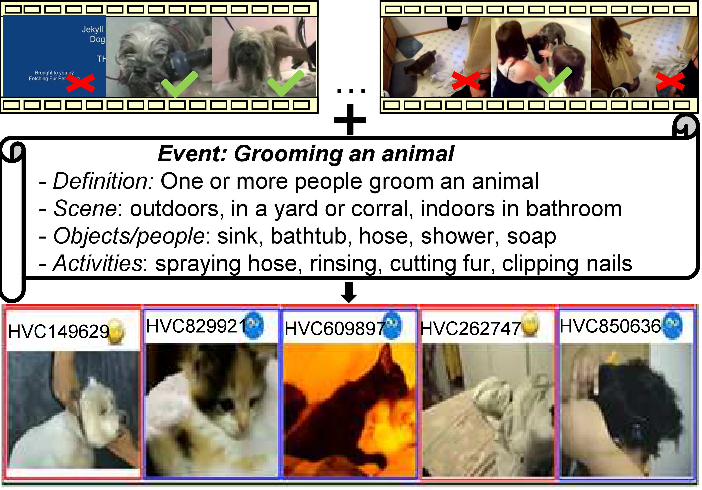
\includegraphics[width=1\textwidth]{figure_1.pdf}
	\caption{Event ``Grooming an animal'' in the TRECVID MED 2012 dataset. The event kit includes example videos and an event description which provides valuable cues to detect that event.}
	\label{figure_1}
\end{figure}

In practice, human \index{human} can recognize a complex event by spotting several evidences in video \cite{bhattacharya2014minimally}. This paper also demonstrated that better performance can be obtained by leveraging positive and negative visual cues selected by humans. Therefore, it is important to automatically detect key evidences for event detection. Several researchers have been working on this direction. Tang \textit{et al.} \cite{tang2012learning} split the video into segments and models key segments and its duration as latent variables. Vahdat \textit{et al.} \cite{vahdat2013compositional} focus on intra-class variation by localizing only the most salient evidence using latent SVM. \index{latent SVM}
Lai \textit{et al.} \cite{lai2014video} detect salient instances in video based on a variant multiple instance learning, \index{multiple instance learning} which was proposed by Yu \textit{et al.} \cite{yu2013propto}. In another work \cite{lai2014recognizing}, they represent static and dynamic instances as sparse features and adopt a learning-to-rank strategy to detect key evidence. In general, these approaches are based on the assumption that segment annotation can be obtained from its video label. However, this is a weak assumption because the importance of each segment is not taken into account. 

\begin{figure}
	\centering
	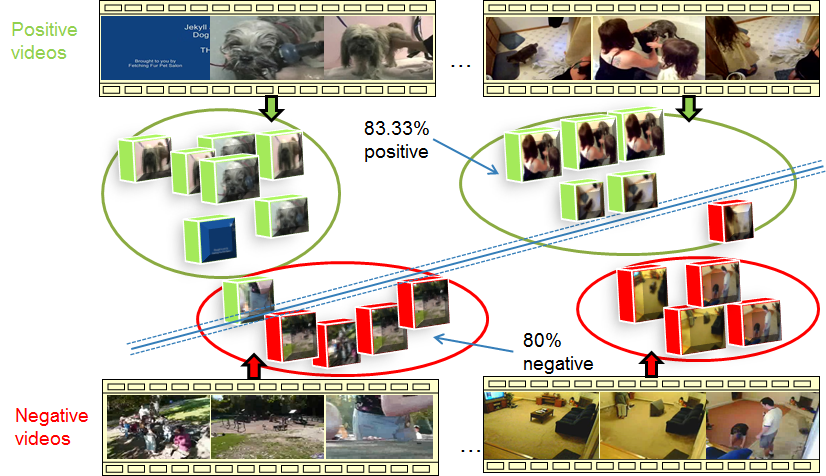
\includegraphics[width=1\textwidth]{pSVM.png}
	\caption{Illustration of pSVM \cite{lai2014recognizing} method. Different from both miSVM and MISVM solutions, pSVM allows some positive instance in the negative bags, which is suitable for real videos.}
	\label{c5_f_psvm}
\end{figure}

On the other hand, the importance of a segment to an event can be obtained by matching its concept-based representation against the evidential description \index{evidential description} of that event. Some works have been using the event description for zero-shot event detection such as in \cite{chen2014event,wu2014zero}. To the best of our knowledge, no work has taken into account this information for detecting key evidence in videos. However, the evidential description of an event provides valuable information to detect that event. Example of an event description (excerpted) is shown in Fig. \ref{figure_1}. 

Motivated by this observation, we propose a new method, Event-driven Multiple Instance Learning (EDMIL), to learn key evidences for complex event detection. We treat each segment as an instance and model it in a multiple instance learning framework \cite{andrews2002support}, where each video is a ``bag''. The instance-event similarity is quantized into different levels of relatedness. Intuitively, the most (ir)relevant instances should have higher (dis)similarities. Therefore, we propose to learn the instance labels by jointly optimize the instance classifier and its related level. We evaluate our proposed method on the large scale TRECVID MED 2012 dataset. Comparing to other instance-based learning methods such as \cite{andrews2002support,lai2014video}, our method achieves a superior performance.

The remaining of this chapter is organized as follows. In the next section, we present the method to calculate the instance-event similarity. Our proposed solution is introduced in Section \ref{c5_method}. The experiments and results are shown in Section \ref{c5_experiment}. Finally, Section \ref{c5_conclusion} concludes this work.
\index{instance-event similarity}

\section{Instance-Event Similarity}
\label{instance_event_similarity}
In order to calculate the similarity between an instance and an event, we adopt a concept expansion strategy as in \cite{chen2014event}. Our method is similar in spirit, however, we apply at instance level which is more accurate. The outline of our method is illustrated in Fig. \ref{c5_figure_2} and it consists of four steps.

\textbf{Step 1: Concept detection.} We use the concept collection that proposed in \cite{zhou2014learning} to cover a wide range of concept that can appear in realistic videos. This collection contains C = 1183 categories including 205 scene categories from the Places Database\cite{zhou2014learning} and 978 object categories from the ImageNet 2012\cite{deng2009imagenet}. The concept detection part is done by using the provided pre-trained model\footnote{http://places.csail.mit.edu}. To detect concept for the whole segment, we detect concept at sample frames and make the average aggregation. \index{concept detection} \index{imagenet} \index{places database}

\textbf{Step 2: Event representation.} We use standard natural language processing techniques to create the text-based event representation. At first, the event description is pre-processed by removing stop words and lemmatizing. It is then converted into a bag-of-words representation, where the dictionary is obtained from the English Wikipedia corpus. Tf-idf weighting scheme is also employed to put a higher weight on frequent as well as rare words.\index{event representation} \index{tf-idf} \index{lemmatization} \index{wikipedia}

\textbf{Step 3: Concept-event similarity.} To resolve the mismatch between words in the concept collection and event description, we adopt the concept expansion strategy \cite{chen2014event}. For each concept category, we add the 10 most similar concepts obtained from word2vec\cite{mikolov2013efficient} model\footnote{https://code.google.com/p/word2vec} to expand this category. It is then represented by a bag-of-words vector with tf-idf weights. Based on this representation, we can calculate the cosine similarity $s_{c}^{e}$ between each concept category and the event description. Table \ref{table1} shows top five most relevant concepts for some events on the MED 2012 dataset. \index{work2vec} \index{tf-idf} 

\textbf{Step 4: Instance-event similarity.} Having obtained the concept score $x_{c}$ at each segment and the concept-event similarity as in Step 1 and Step 3, the instance-event similarity is calculated using the cosine similarity:
\begin{equation}
\label{eq1}
S_{i}^{e}=\frac{\sum_{c=1}^{C}s_{c}^{e}x_{c}}{\sqrt{\sum_{c=1}^{C}(s_{c}^{e})^{2}}\sqrt{\sum_{c=1}^{C}(x_{c})^{2}}},
\end{equation}
\begin{figure}
	\centering
	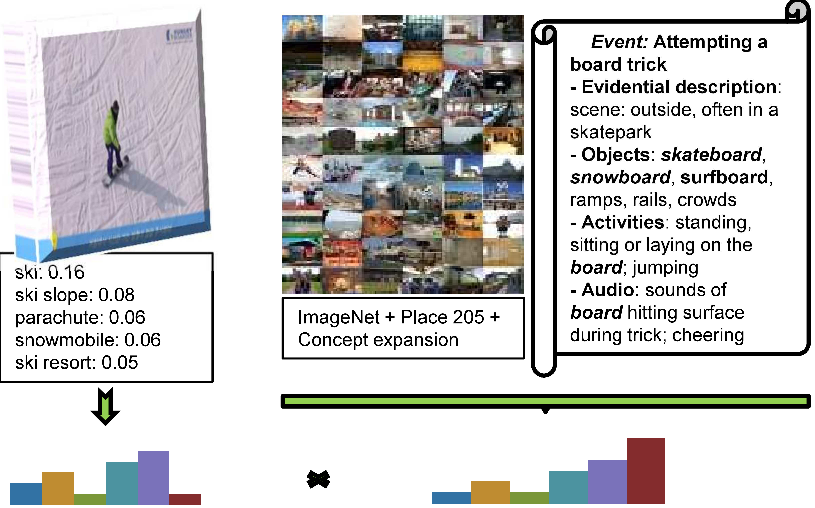
\includegraphics[width=1\textwidth]{figure_2.pdf}
	\caption{Outline of our method to calculate the instance-event similarity. Note that the concept expansion technique can bridge concept ``ski'' in the instance segment to the evidential description.}
	\label{c5_figure_2}
\end{figure}


\begin{table}
		\renewcommand{\arraystretch}{1.3}
		\centering
		\caption{Top five concepts discovered by our system for 25 events in the MED 2012 dataset.}
	\begin{tabular}{|c|l|}
		\toprule
		\textbf{Event ID} & \multicolumn{1}{c|}{\textbf{Top five importance concepts discovered by our system}} \\ \midrule
		E001              & Ski, slide rule, ski resort, ski mask, ice skating rink                             \\ \midrule
		E002              & Meat loaf, white shark, food court, pop bottle, cleaver                             \\ \midrule
		E003              & Anemone fish, pole, raft, sturgeon, boat deck                                       \\ \midrule
		E004              & Groom, bridegroom, banquet hall, gown, altar                                        \\ \midrule
		E005              & Jigsaw puzzle, bamboo forest, carpenter's kit, thatch, wooden spoon                 \\ \midrule
		E006              & Table lamp, lampshade, torch, candle, custard apple                                 \\ \midrule
		E007              & Recreational vehicle, car wheel, amphibian, scooter, sports car                     \\ \midrule
		E008              & Monitor, chime, bell, whistle, ballroom                                             \\ \midrule
		E009              & Recreational vehicle, amphibian, tank, car wheel, motor scooter                     \\ \midrule
		E010              & Nail, bathtub, shower, fur coat, washbashin                                         \\ \midrule
		E011              & Pizza, bagel, meat loaf, cheeseburger, vegetable garden                             \\ \midrule
		E012              & Recreational vehicle, amphibian, tank, sports car, freight car                      \\ \midrule
		E013              & Playground, volleyball, picnic area, sports car, table lamp                         \\ \midrule
		E014              & Toaster, dish washer, washing machine, refrigerator, space heater                   \\ \midrule
		E015              & Sewing machine, dragonfly, syringe, clothing store, construction site               \\ \midrule
		E016              & Digital watch, classroom, CD player, crossword, stopwatch                           \\ \midrule
		E017              & Tray, game room, cassette player, CD player, waiting room                           \\ \midrule
		E018              & Backpack, walking stick, pop bottle, sleeping bag, plastic bag                      \\ \midrule
		E019              & Tile roof, mortar, nail, jigsaw puzzle, drumstick                                   \\ \midrule
		E020              & Ballpoint, pencil box, rubber eraser, quill pen, pencil sharpener                   \\ \midrule
		E021              & Tricycle, mountain bike, scooter, bicycle-built-for-two, unicycle                   \\ \midrule
		E022              & Toaster, refrigerator, dish washer, washing machine, space heater                   \\ \midrule
		E023              & Schipperke, otter hound, bluestick, collie, Tibetan terrier                         \\ \midrule
		E024              & Forest path, cellular telephone, phone booth, platform, dial phone                  \\ \midrule
		E025              & Boxing ring, fairway, hand-held computer, bell cote, chime                          \\ \bottomrule
	\end{tabular}
		\label{table1}
\end{table}

\section{Event-Driven Multiple Instance Learning}
\label{c5_method}

\subsection{Problem Formalization} Suppose we have $V$ training videos, and $I_{v}$ instances in video $v$. We can calculate the similarity $S_{iv}^{e}$ between an instance $iv$ to a particular event $e$ using Eq. (\ref{eq1}). Suppose there is R level of relatedness from an instance to an event. We define two predict functions for positive and negative instances at level $r$ as follows.
\begin{equation}
\label{eq2}
P_{pos}(S_{iv}^{e},r) = 
\begin{cases}
1,& \text{if } Rank(S_{iv}^{e}) \leq r \\
-1,              & \text{otherwise}
\end{cases}\text{, and}
\end{equation}

\begin{equation}
\label{eq3}
P_{neg}(S_{iv}^{e},r) = 
\begin{cases}
-1,& \text{if } Rank(S_{iv}^{e}) \leq r \\
1,              & \text{otherwise}
\end{cases}\text{, }
\end{equation}
where $Rank(.)$ is the function to quantize a similarity into a related level. Note that smaller value of $r$ results a higher confidence in the predict functions. We now learn the parameters of the instance classifier jointly with the related level $r$ by optimizing the following objective function: \index{instance classifier}

\begin{equation}
\label{eq4}
\begin{split}
\min_{\textbf{w},b,y,r} \frac{1}{2} \left \| \textbf{w} \right \|^{2} + C_{f} \sum_{v=1}^{V}\sum_{i=1}^{I_{v}}L_{f}\left ( y_{iv}, \textbf{w}^{T}\textbf{x}_{iv}+b \right ) \\
+ C_{p} \sum_{v=1}^{V}\sum_{i=1}^{I_{v}}L_{p}\left ( y_{iv}, P(S_{iv}^{e},r) \right ).
\end{split}
\end{equation}
$C_{f}$ and $C_{p}$ are cost parameters to control the influence of each loss function. Note that in the special case where $C_{p}=0$, the above formulation becomes a classic large-margin problem. $L_{f}(.)$ and $L_{p}(.)$ are two loss functions that will be jointly minimized. The first loss function minimizes the loss due to the classification mismatch based on the instance feature. The second one minimizes the loss due to the prediction obtained from the prior knowledge. Intuitively, when the related level $r$ increases, the first loss will also tend to increase while the second loss will become smaller, and vice versa. $L_{f}(.)$ and $L_{p}(.)$ can be any loss function. Throughout this work, we use the standard hinge-loss function for $L_{f}(.)$: \index{hinge-loss function}
$L_{f}\left ( y_{iv},\textbf{w}^{T}\textbf{x}_{iv}+b \right )=\text{max}(0,1-y_{iv}(\textbf{w}^{T}\textbf{x}_{iv}+b)),$
and the $L_{p}(.)$ function is defined so that it will penalize more on the high confident predictions:
\begin{center}
$L_{p}\left ( y_{iv}, P(S_{iv}^{e},r) \right )= 
\begin{cases}
S_{iv}^{e},& \text{if } P(S_{iv}^{e},r) \neq y_{iv} \\
0,              & \text{otherwise}
\end{cases}.$
\end{center}

\subsection{Optimization Procedure} \index{optimization}
The optimization problem in Eq. (\ref{eq4}) is a mixed-integer program which is not convex. In order to solve this problem, we apply the alternating optimization strategy to search for a suboptimal solution:
\begin{enumerate}
	\item{} Fix instance labels $y_{iv}$ and solve for \textbf{w} and \textit{b}. By fixing $y_{iv}$, the optimization problem becomes a classic SVM:
	\begin{center}
	$\min\limits_{\textbf{w},b}$ $\frac{1}{2} \left \| \textbf{w} \right \|^{2} + C_{f} \sum_{v=1}^{V}\sum_{i=1}^{I_{v}}L_{f}\left ( y_{iv}, \textbf{w}^{T}\textbf{x}_{iv}+b \right )$. 
	\end{center}
	Thus it can be solved using a regular SVM solver.
	
	\item{} Fix \textbf{w} and \textit{b}, solve for $r$ and update $y_{iv}$. The problem now becomes: 
	
	\begin{center}
	$\min\limits_{y,r} C_{f} \sum_{v=1}^{V}\sum_{i=1}^{I_{v}}L_{f}\left ( y_{iv}, \textbf{w}^{T}\textbf{x}_{iv}+b \right ) 
	+ C_{p} \sum_{v=1}^{V}\sum_{i=1}^{I_{v}}L_{p}\left ( y_{iv}, P(S_{iv}^{e},r) \right ).$
	\end{center}
		
	%\begin{equation}
	%\label{eq7}
	%\begin{split}
	%\min_{y,r} C_{f} \sum_{v=1}^{V}\sum_{i=1}^{I_{m}}L_{f}\left ( %y_{iv}, \textbf{w}^{T}\textbf{x}_{iv}+b \right ) \\
	%+ C_{p} \sum_{v=1}^{V}\sum_{i=1}^{I_{m}}L_{p}\left ( y_{iv}, %P(S_{iv}^{e},r) \right ).
	%\end{split}
	%\end{equation}
	We propose a greedy strategy to solve for this problem. At first, we iterate through all level of relatedness to search for the optimal $r$ by finding the minimum total loss when updating $y_{iv}$ using Eq. (\ref{eq2}, \ref{eq3}). Because the most positive and negative instances will be selected first, there will be a higher possibility to correct mismatched labels that were learned in the previous step. Lastly we update instance labels using Eq. (\ref{eq2}, \ref{eq3}) with the optimal $r$. \index{greedy strategy}
	
\end{enumerate}

Because this is not a convex optimization problem, the initialized values of $y_{iv}$ should be carefully selected. To this end, we use the same initilization method as in \cite{andrews2002support,lai2014video}, where instance labels are same with its ``bag'' (video) label. \index{convex optimization}

It is also worth noted that the optimization framework only keeps updating the instance labels while the instance features are unchanged. Thus it is a good practice to use the pre-computed kernel technique for optimizing \textbf{w} and \textit{b}. In fact, although our method is more complex, it only takes around 5 minutes for training one model, compared to 40 minutes that was reported in \cite{lai2014video}. 
\section{Experiment}
\label{c5_experiment}
\subsection{Dataset} To evaluate our proposed method, we conducted experiments on the large scale TRECVID MED 2012 dataset\footnote{http://www.nist.gov/itl/iad/mig/med12.cfm}. This dataset provides the definition for 25 complex events. The first ten event names are listed in Table \ref{table1}. We follow the setting by \cite{lai2014video} to divide this video collection into training and testing parts. These parts contain 3,878 and 1,938 videos respectively.

\subsection{Experimental Setup} At first, original videos are scaled down to 320 x 240 with keeping the aspect ratio. Key frames are sampled at every 2 seconds from the resized video. The segment length is set to 8 seconds as suggested in \cite{vahdat2013compositional}. To extract feature for each segment, we use the Improved Dense Trajectories feature proposed by Wang and Schmid \cite{wang2013action}. Motion Boundary Histogram (MBH) is used to represent extracted trajectories because it can handle camera motion, which is prevalent in realistic videos. For learning, we use our framework jointly with the linear SVM. The cost parameters $C_{f}$ and $C_{p}$ are selected by cross-validation in the range of $\{0.1, 1, 10, 100\}$. At the testing step, video-level score is obtained by averaging over all instance scores. Finally we use the standard evaluation metric on MED, Mean Average Precision (mAP), to report the performance.

\begin{figure}
	\centering
	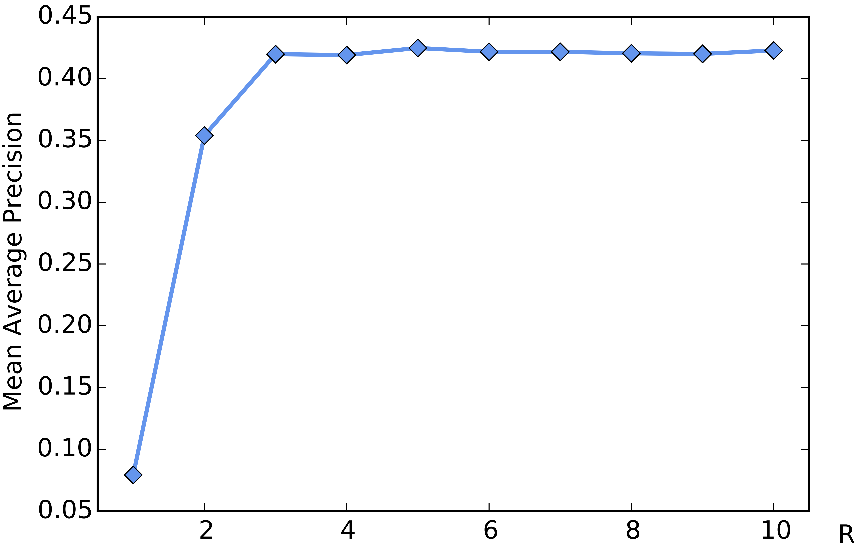
\includegraphics[width=1\textwidth]{figure_3.pdf}
	\caption{Optimal number of related levels.}
	\label{figure_3}
\end{figure}


\subsection{Baseline Methods} We compare our methods with following baselines: miSVM, MISVM \cite{andrews2002support}, VideoBOW and pSVM \cite{lai2014video}. At first, because our method is based on the Multiple Instance Learning (MIL) framework, we evaluate two MIL solutions: miSVM and MISVM that were proposed by the authors in \cite{andrews2002support}. The VideoBOW method is the standard approach where local features are aggregated from the whole video. We also compare our method with the recently proposed pSVM which was adopted in \cite{lai2014video} for TRECVID MED. For all the baseline methods, except VideoBOW, we utilize the codes provided by the authors to test with our features.


\subsection{Experimental Results}
At first, we conduct experiments to find the optimal value of R. We select R in the range from 1 to 10. The overall performance is shown in Fig. \ref{figure_3}. We obtain the peak performance with R around 5. Small values of R tend to get low performances. This indicates that the prediction of prior knowledge is not always good, and learning jointly with instance features is necessary. The performance becomes saturated when R > 5. Therefore, we fix the value of R to 5 for further experiments.

\subsubsection{On The MED 2012 dataset}
The performance of each baseline method as well as our method (EDMIL) are shown in Fig. \ref{figure_4}. Our method significantly outperforms other baselines. For the best baseline, our method relatively outperforms by 10\%. Our instance-based classifier can also provide key evidences for event detection. Example of true positive and false positive key evidences detected by our system can be seen in Fig. \ref{figure_5} and Fig. \ref{figure_6} respectively. 

\begin{figure*}
	\centering
	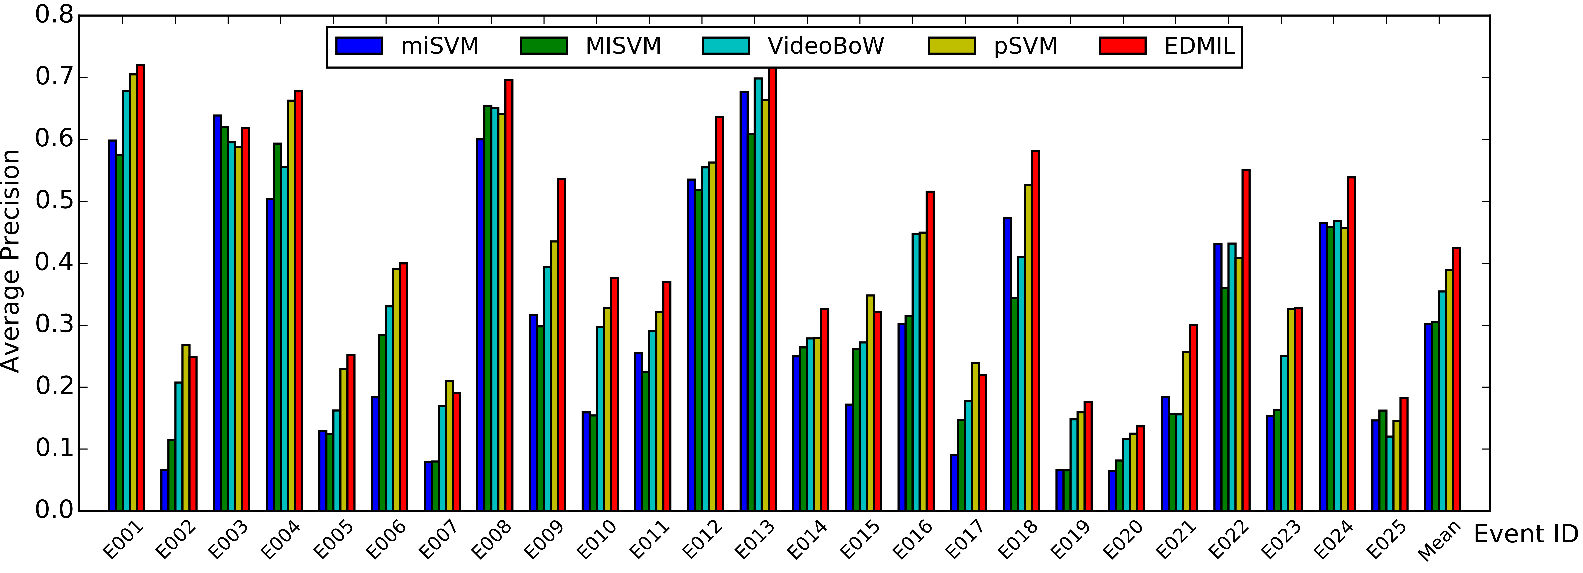
\includegraphics[width=1.1\textwidth]{figure_4.pdf}
	\caption{Evaluation results of 25 events in the TRECVID MED 2012 dataset. The mean APs are 0.3015 (miSVM), 0.3051 (MISVM), 0.3544 (VideoBOW), 0.3890 (pSVM) and 0.4246 (Ours).}
	\label{figure_4}
\end{figure*}

\subsubsection{On The MED 2011 dataset}
For the MED 2011 dataset, we also compare our proposed method with our two previous works: Segment-based Representation (SB) and Sum-Max Video Pooling (SM) at segment length of 8 s. The results are shown in Fig. \ref{med11_sum}.

\begin{figure}
	\centering
	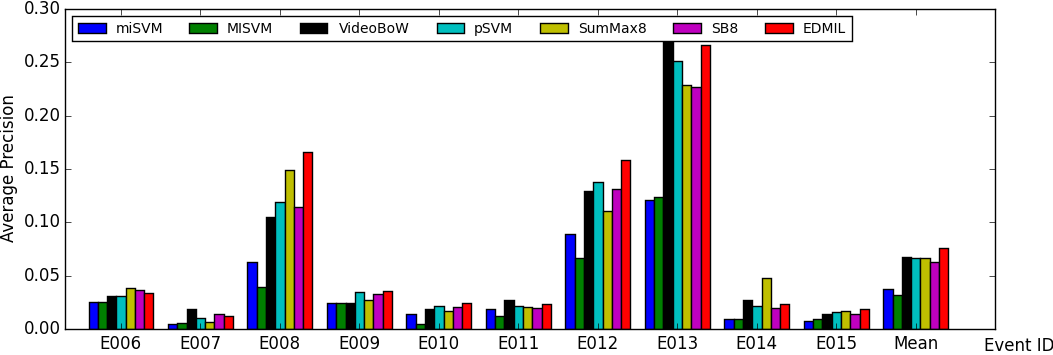
\includegraphics[width=1\textwidth]{med11_sum.png}
	\caption{Evaluation results of 10 events in the TRECVID MED 2011 dataset using average aggregation. The mean APs are 0.0378 (miSVM), 0.0322 (MISVM), 0.0674 (VideoBOW), 0.0666 (pSVM), 0.0663 (SM8), 0.0630 (SB8), \textbf{0.0761} (\textbf{Ours}).}
	\label{med11_sum}
\end{figure}

Our proposed EDMIL approach achieves the best performance while p-SVM only has a comparable performance with the VideoBOW. Our segment-based approach (SB) does not perform well. The reason is that we used the average aggregation over all segments of the video at the testing step. We further conduct experiment with a new testing strategy: choose the max segment score as the video score. The result of this experiment is shown on Fig. \ref{med11_max}. The max aggregation strategy performs better than the average aggregation by a margin. The performance gain can be seen in Fig. \ref{med11_gain}. 

\begin{figure}
	\centering
	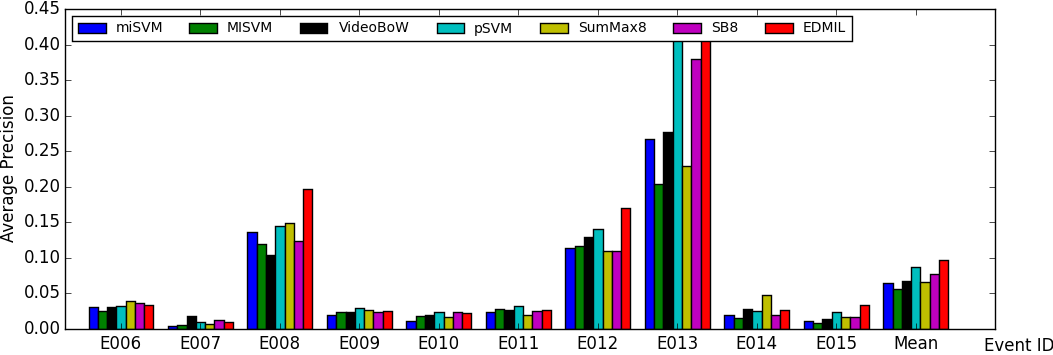
\includegraphics[width=1\textwidth]{med11_max.png}
	\caption{Evaluation results of 10 events in the TRECVID MED 2011 dataset using max aggregation. The mean APs are 0.0640 (miSVM), 0.0564 (MISVM), 0.0674 (VideoBOW), 0.0870 (pSVM), 0.0663 (SM8), 0.0770 (SB8), \textbf{0.0968} (\textbf{Ours}).}
	\label{med11_max}
\end{figure}

\begin{figure}
	\centering
	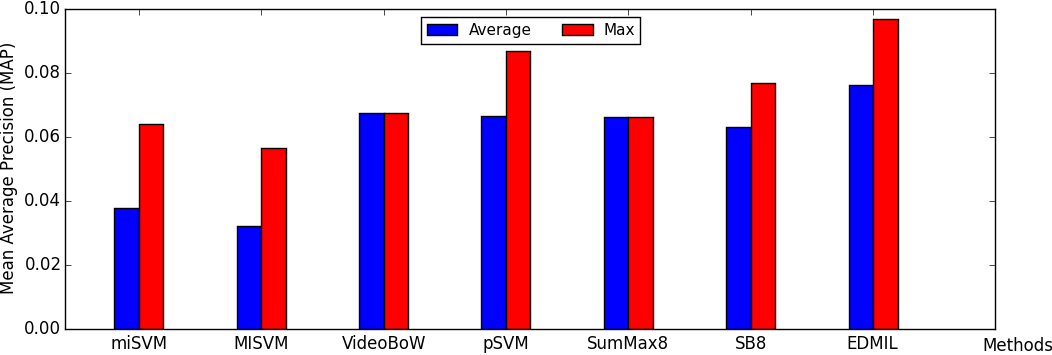
\includegraphics[width=1\textwidth]{med11_gain.png}
	\caption{The top 6 key evidences detected by our system for the event ``Attempting board trick''. The dominance of ski-related instances is reasonable.}
	\label{med11_gain}
\end{figure}

\begin{figure}
	\centering
	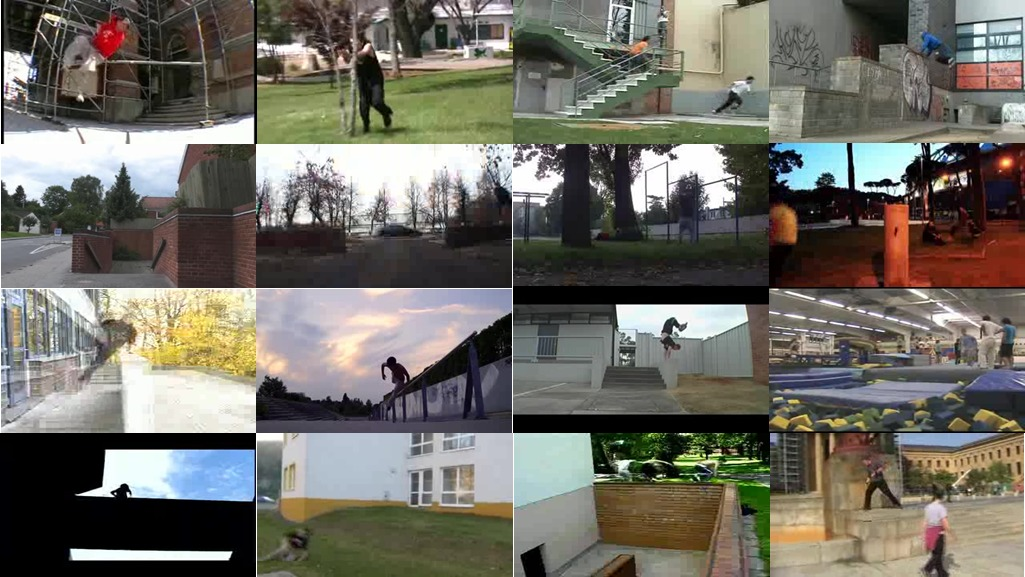
\includegraphics[width=1\textwidth]{parkour.jpg}
	\caption{The top 16 key evidences detected by our system for the event ``Parkour''.}
	\label{figure_5}
\end{figure}

\begin{figure}
	\centering
	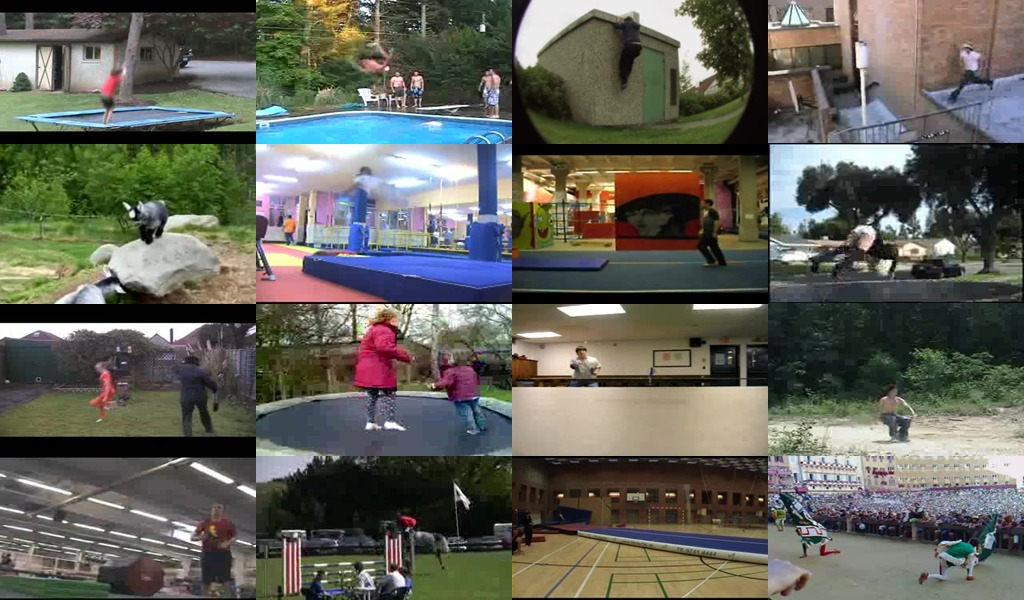
\includegraphics[width=1\textwidth]{parkour_neg.jpg}
	\caption{The top 16 key false positive evidences detected by our system for the event ``Parkour''.}
	\label{figure_6}
\end{figure}

\section{Conclusion}
\label{c5_conclusion}
We propose a new method to detect event in videos from its key evidences. Our method differs from others in that we utilize the evidential description provided for each event. Given this supportive information, we search for key evidences by jointly optimizing with instance feature in a variant of multiple instance learning framework. As a result, we obtained a superior event detection performance.

